% !TeX root = Stageportfolio.tex

\begin{landscape}
	
	\begin{tabularx}{1.56\textwidth}{|X|}
		\hline
		Naam stagair:  Kevin Truyaert  \\
		Tel.: 0495/928460 \hspace{3cm} e-mail: kevin.truyaert@student.kuleuven.be  \\
		Naam en adres opleidingsinstituut:  KU Leuven Campus Kulak Kortrijk, Etienne-Sabbelaan 53, 8800 Kortrijk  \\
		Naam directie: \\
		Naam stagecoördinator:  David Dudal \\
		\hline
	\end{tabularx}
	\vspace*{-0.4cm}
\section{Observatie- en stageplanning}
\vspace*{-0.3cm}\subsection{Observatieplanning}
\subsubsection{Kulak (LIO)}%
%\parskip 
%\vspace{\parskip}
\begin{minipage}[b]{\textwidth}
	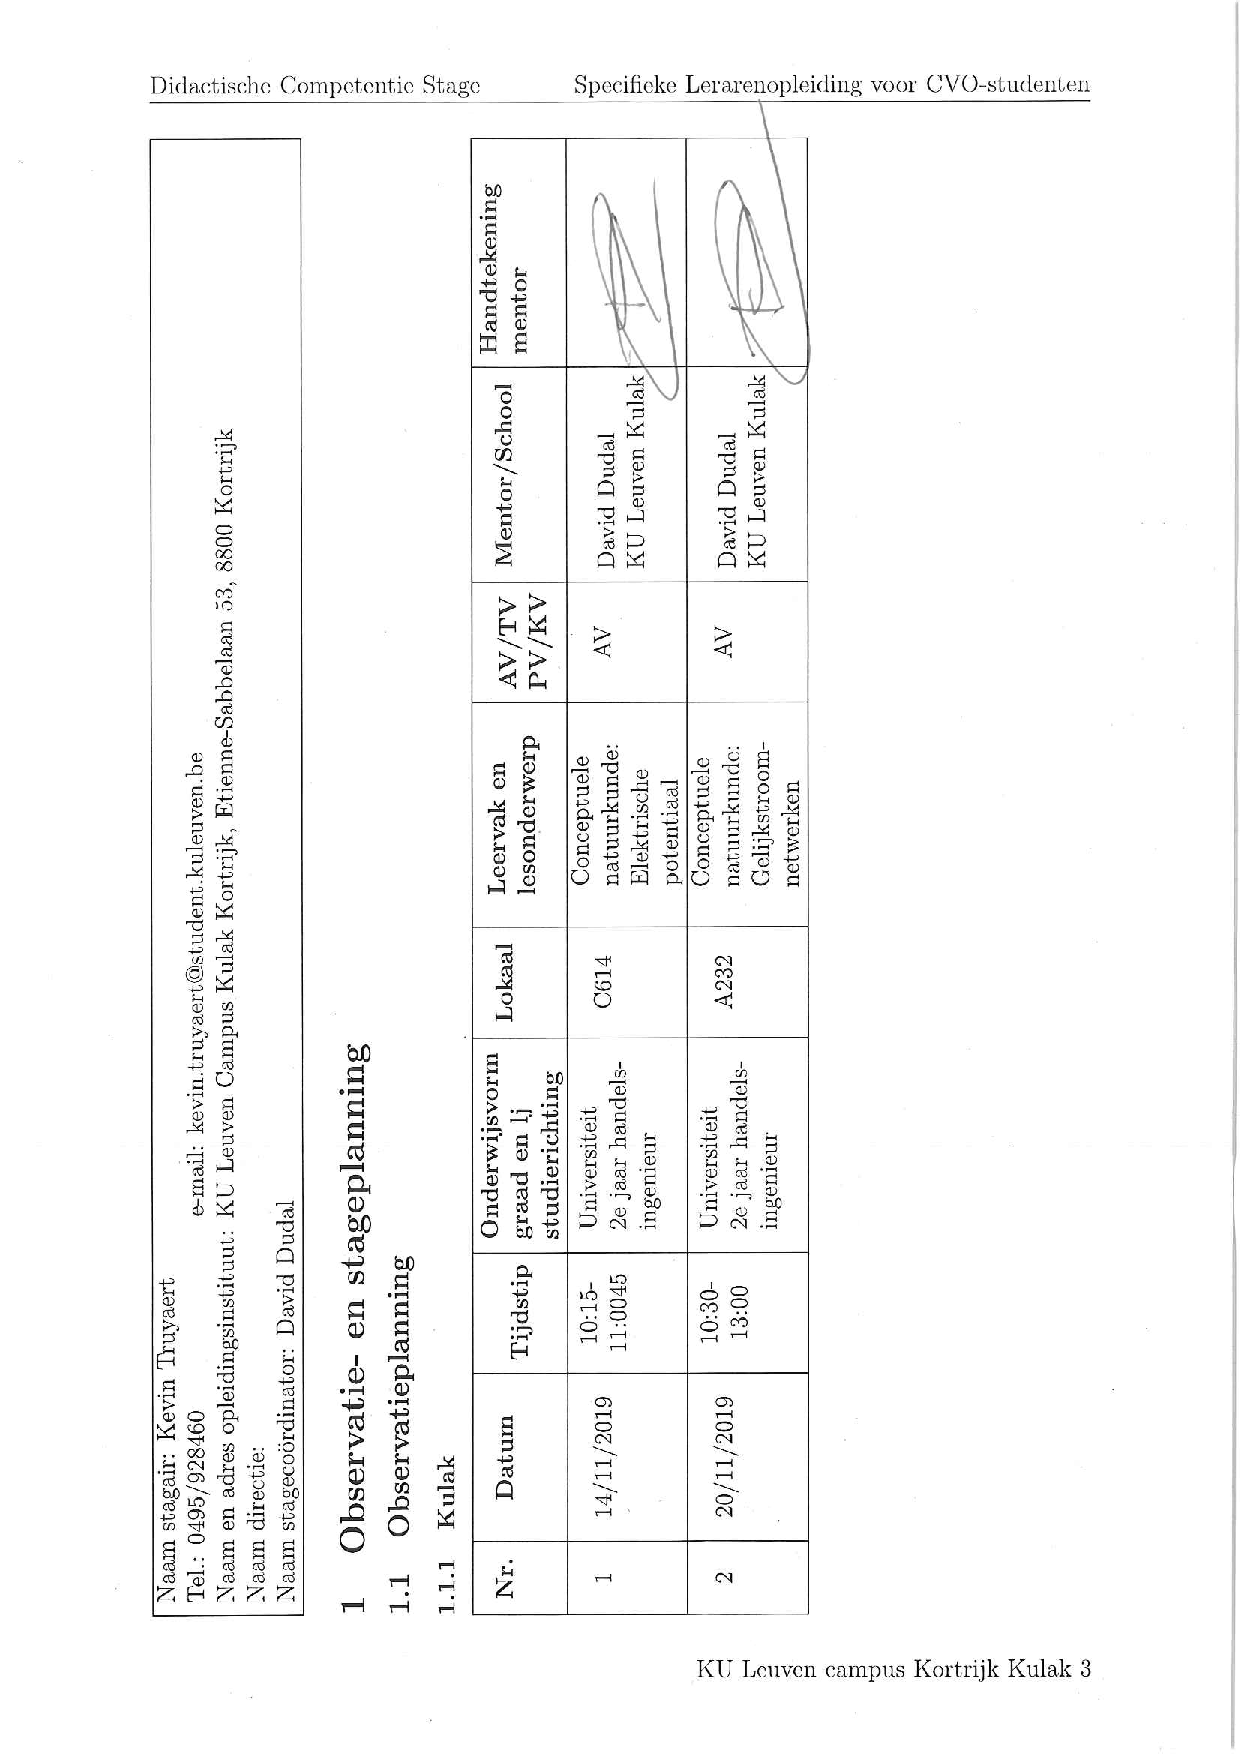
\includepdf[scale = 0.85,pages = 1,trim={7.8cm 2cm 7.3cm 2cm} ,clip,pagecommand = ]{VerslagenDavid2}
\end{minipage}

%\begin{tabularx}{1.56\textwidth}{|C{0.05\textwidth}|C{0.15\textwidth}|C{0.1\textwidth}|C{0.2\textwidth}|C{0.09\textwidth}|C{0.21\textwidth}|C{0.1\textwidth}|C{0.2\textwidth}|X|}
%	\hline
%	\textbf{Nr.} & \textbf{Datum} & \textbf{Tijdstip} & \textbf{\begin{tabular}[C]{@{}l@{}}Onderwijsvorm\\ graad en lj\\ studierichting\end{tabular}} & \textbf{Lokaal} &\textbf{\begin{tabular}[C]{@{}l@{}} Leervak en\\ lesonderwerp \end{tabular}} & \textbf{\begin{tabular}[C]{@{}l@{}}AV/TV\\PV/KV\end{tabular}} & \textbf{Mentor/School} & \textbf{\begin{tabular}[C]{@{}l@{}} Handtekening\\mentor\end{tabular}}\\ \hline
%	1 & 14/11/2019 & 10:15-11:0045 &\begin{tabular}[C]{@{}l@{}}Universiteit\\2e jaar handels-\\ingenieur\end{tabular} & C614 & \begin{tabular}[C]{@{}l@{}}Conceptuele\\ natuurkunde:\\ Elektrische\\ potentiaal \end{tabular} & AV & \begin{tabular}[C]{@{}l@{}}David Dudal\\ KU Leuven Kulak \end{tabular} & \\ \hline
%	2 & 20/11/2019 & 10:30-13:00 &\begin{tabular}[C]{@{}l@{}}Universiteit\\2e jaar handels-\\ingenieur\end{tabular} & A232 & \begin{tabular}[C]{@{}l@{}}Conceptuele\\ natuurkunde:\\ Gelijkstroom-\\netwerken\end{tabular} & AV & \begin{tabular}[C]{@{}l@{}}David Dudal\\ KU Leuven Kulak \end{tabular} & \\ \hline
%\end{tabularx}
	
\newpage
\subsection{Actieve stage}
		\subsubsection{Kulak (LIO)}
		
		\begin{minipage}[t][10cm][t]{0.5\textwidth}
			\includepdf[scale = 0.85,pages = 2,trim={4cm 2cm 6cm 1.8cm} ,clip,pagecommand = ]{VerslagenDavid2}
		\end{minipage}
%	\begin{tabularx}{1.56\textwidth}{|C{0.15\textwidth}|C{0.14\textwidth}|C{0.14\textwidth}|C{0.1\textwidth}|C{0.1\textwidth}|C{0.05\textwidth}|C{0.35\textwidth}|X|}
%		\hline
%		\textbf{Datum} & \textbf{Vestiging} & \textbf{\begin{tabular}[C]{@{}l@{}}Aantal\\ stage-uren\end{tabular}} & \textbf{\begin{tabular}[C]{@{}l@{}}Uur \end{tabular}}    & \textbf{Lokaal}& \textbf{\begin{tabular}[C]{@{}l@{}}AV\\TV\\PV\\KV\end{tabular}}& \textbf{\begin{tabular}[C]{@{}l@{}}Onderwijsvorm\\ graad en lj\\ Vak en lesonderwerp\end{tabular}}  &  \textbf{\begin{tabular}[C]{@{}l@{}}Naam vakmentor\\ + handtekening\end{tabular} } \\ \hline
%		27/11/2019 & Kulak & 1-3 & 10:30-13:00 & A352 & AV & Universiteit\newline 2e jaar Handelsingenieur\newline Conceptuele natuurkunde\newline werkzitting elektromagnetisme & \\ 
%\hline
%		4/12/2019 & Kulak & 4-5 & 10:30-13:00 & A352 & AV & Universiteit\newline 2e jaar Handelsingenieur\newline Conceptuele natuurkunde\newline werkzitting elektromagnetisme & \\ \hline
%		11/12/2019 & Kulak & 6-8 & 10:30-13:00 & A352 & AV & Universiteit\newline 2e jaar Handelsingenieur\newline Conceptuele natuurkunde\newline werkzitting elektromagnetisme & \\ \hline
%		19/12/2019 & Kulak & 9-10 & 10:00-12:30 & A352 & AV & Universiteit\newline 2e jaar Handelsingenieur\newline Conceptuele natuurkunde\newline werkzitting elektromagnetisme & \\ \hline
%	%	 &  &  &  &  &  &  & \\ \hline
%	\end{tabularx}
%		


		
\end{landscape}		
		
